%\chapter*{Отчет}
\section*{Тренировочное задание}

На рисунке \ref{p1} изображен ресурсный лист, заполненный в соответствии с 1ым вариантом.
\begin{figure}[!h]
	\centering
	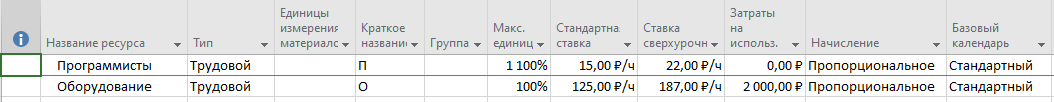
\includegraphics[width=1\linewidth]{inc/img/1.png}
	\caption{Ресурсный лист}
	\label{p1}
\end{figure}

На рисунке \ref{p2} изображена полученная диаграмма Ганта.
\begin{figure}[!h]
	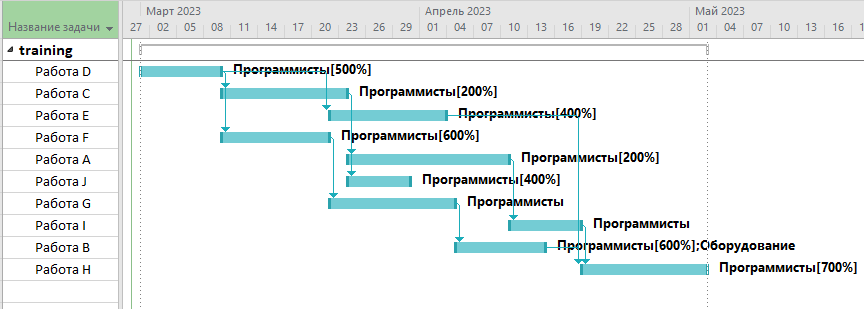
\includegraphics[width=1\linewidth]{inc/img/2.png}
	\caption{Диаграмма Ганта}
	\label{p2}
\end{figure}

На рисунке \ref{p3} можно увидеть необходимый бюджет проекта.
\begin{figure}[!h]
	\centering
	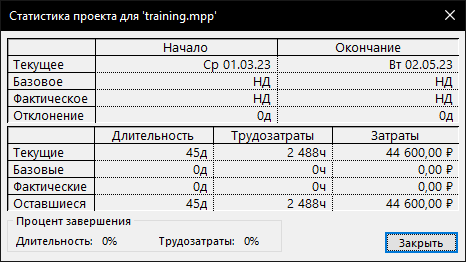
\includegraphics[width=0.7\linewidth]{inc/img/3.png}
	\caption{Бюджет проекта}
	\label{p3}
\end{figure}

\newpage
При этом оборудование обошлось в 8 тысяч (рис. \ref{p33})
\begin{figure}[!h]
	\centering
	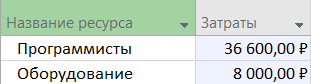
\includegraphics[width=0.7\linewidth]{inc/img/3.0.png}
	\caption{Затраты}
	\label{p33}
\end{figure}

\section*{Лабораторная работа}
\textbf{Содержание проекта:} Команда разработчиков из \textbf{16 человек} занимается созданием карты города на основе собственного модуля отображения. Проект должен быть завершен в течение \textbf{6 месяцев}. Бюджет проекта: 50 000 рублей.

\subsection*{Задание №1: Создание списка ресурсов}

На рисунке \ref{p4} изображена информация о ресурсах, используемых в проекте.
\begin{figure}[!h]
	\centering
	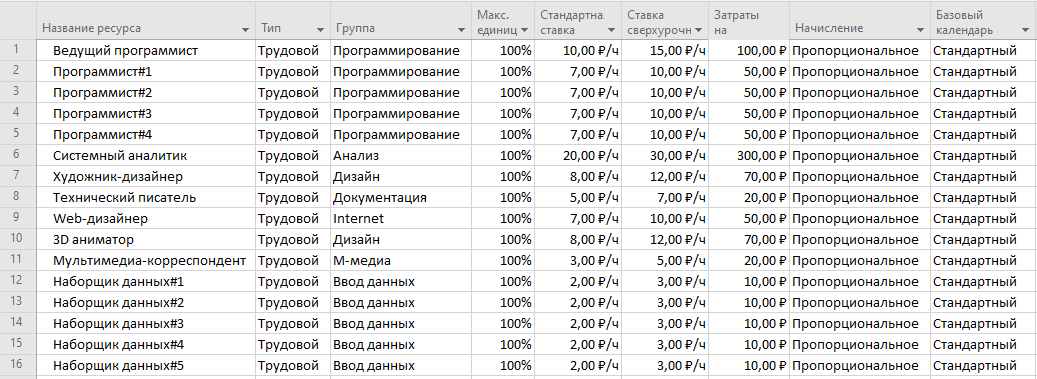
\includegraphics[width=1\linewidth]{inc/img/4.png}
	\caption{Информация о ресурсах}
	\label{p4}
\end{figure}

\newpage
\subsection*{Задание №2: Назначение ресурсов задачам}
В задании №2 нужно было назначить ресурсы задачам. Результат представлен на рисунке \ref{p5}.
\begin{figure}[!h]
	\centering
	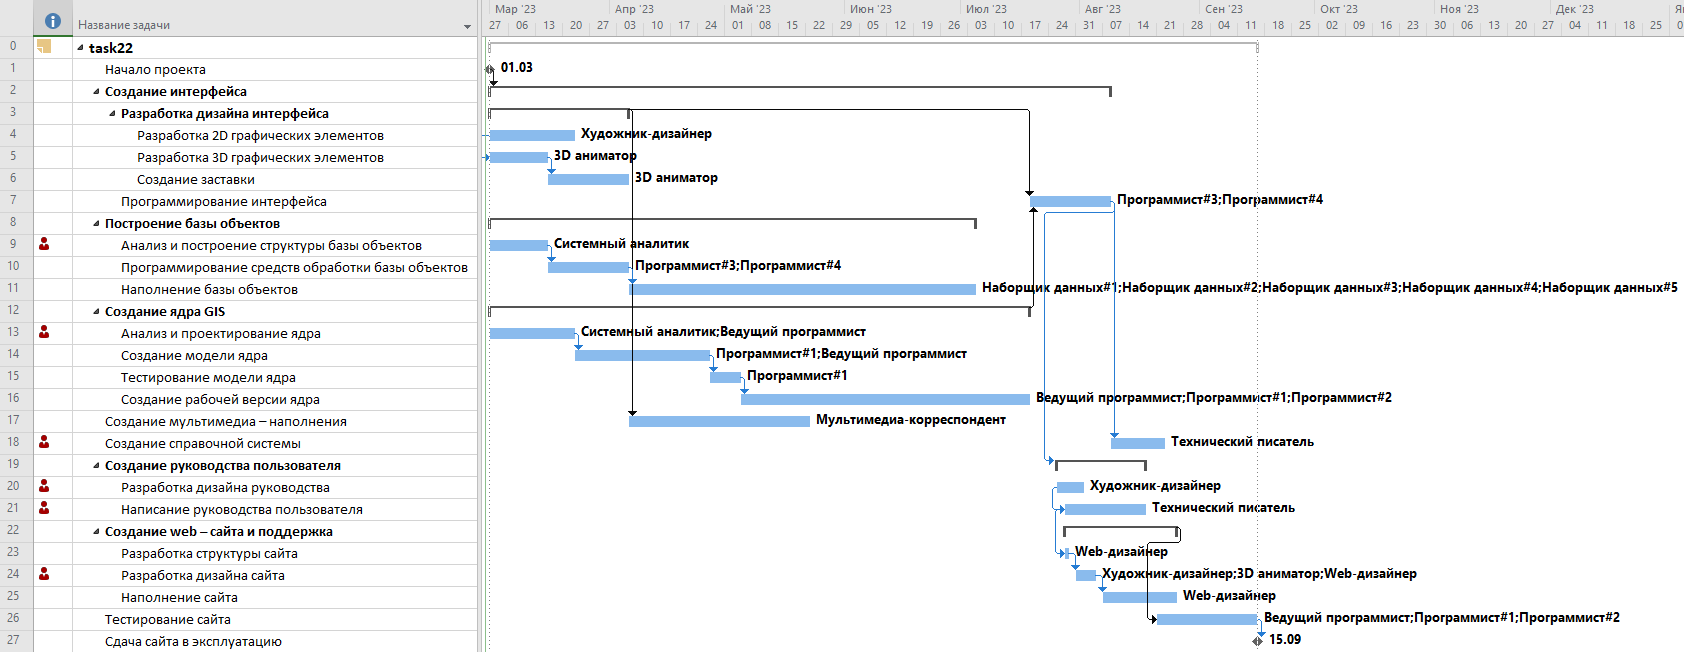
\includegraphics[width=1\linewidth]{inc/img/5.png}
	\caption{Назначение ресурсов задачам}
	\label{p5}
\end{figure}

По диаграмме Ганта видно, что некоторые ресурсы используются для нескольких задач одновременно, что решается переносом соответствующих задач на допустимую дату. На рисунке \ref{p6} изображена исправленная диаграмма Ганта.

\begin{figure}[!h]
	\centering
	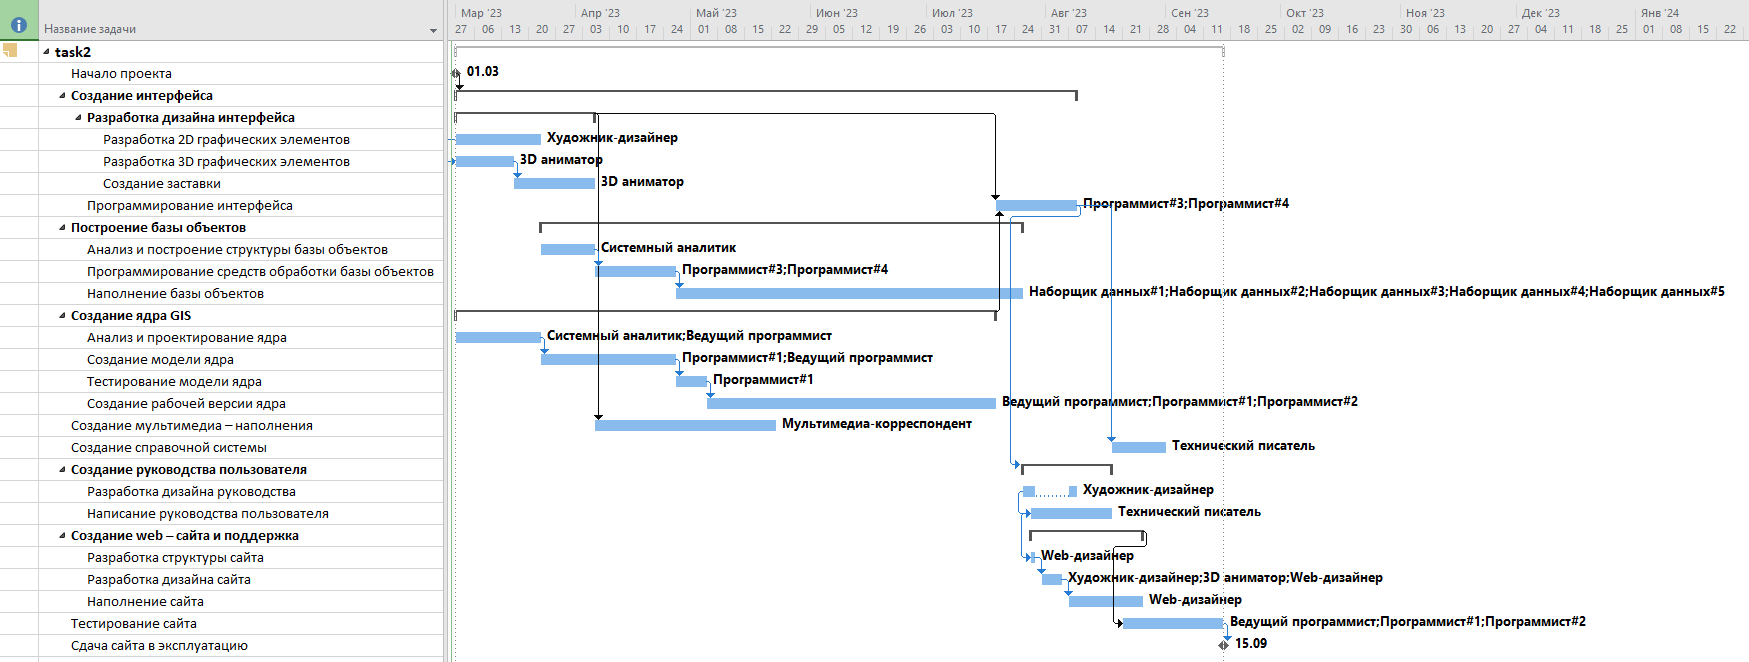
\includegraphics[width=1\linewidth]{inc/img/6.png}
	\caption{Исправленная диаграмма Ганта}
	\label{p6}
\end{figure}

Дополнительный сервер был добавлен как трудовой ресурс, т.к. он арендуется. При этом надо учитывать что он работает 24/7. На рисунке \ref{p66} видно сколько затрат и трудозатрат потребует сервер.

\begin{figure}[!h]
	\centering
	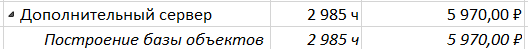
\includegraphics[width=1\linewidth]{inc/img/6.0.png}
	\caption{Затраты на дополнительный сервер}
	\label{p66}
\end{figure}

\newpage
\subsection*{Задание №3: Анализ затрат по группам ресурсов}
В задании №3 нужно было провести структуризацию затрат по группам ресурсов (рис. \ref{p7}).
\begin{figure}[!h]
	\centering
	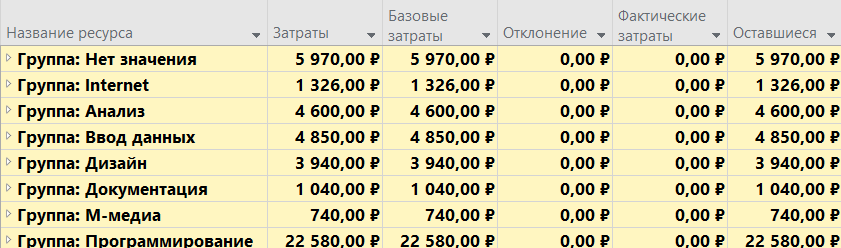
\includegraphics[width=1\linewidth]{inc/img/7.png}
	\caption{Структуризация затрат по группам ресурсов}
	\label{p7}
\end{figure}

На рисунке \ref{d1} изображена диаграмма затрат по группам ресурсов.
\begin{figure}[!h]
\centering
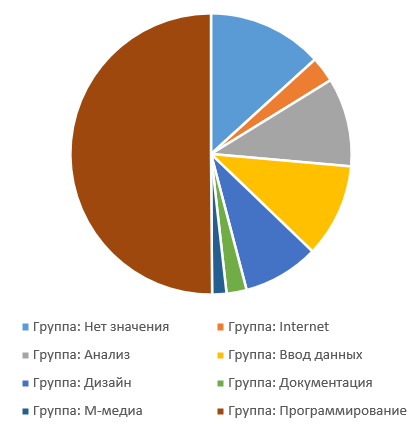
\includegraphics[width=0.6\linewidth]{inc/img/d1.png}
\caption{Диаграмма затрат по группам ресурсов}
\label{d1}
\end{figure}

\newpage
На рисунке \ref{p8} изображена структуризация трудозатрат по группам ресурсов.
\begin{figure}[!h]
	\centering
	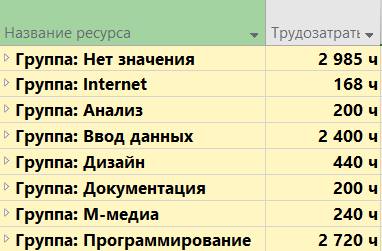
\includegraphics[width=0.6\linewidth]{inc/img/8.png}
	\caption{Структуризация трудозатрат по группам ресурсов}
	\label{p8}
\end{figure}

На рисунке \ref{d2} изображена диаграмма трудозатрат по тем же группам ресурсов.
\begin{figure}[!h]
	\centering
	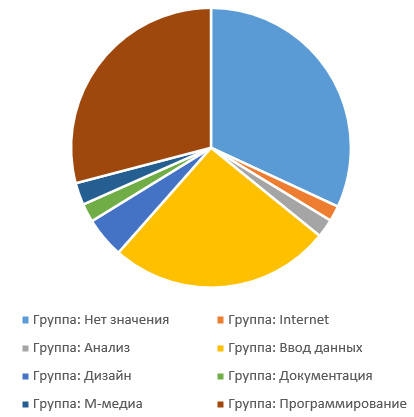
\includegraphics[width=0.6\linewidth]{inc/img/d2.png}
	\caption{Диаграмма трудозатрат по группам ресурсов}
	\label{d2}
\end{figure}

\newpage
На рисунке \ref{p9} представлено сопоставление в логике «Деньги» – «Объем работ» («Затраты – Трудозатраты»)
\begin{figure}[!h]
	\centering
	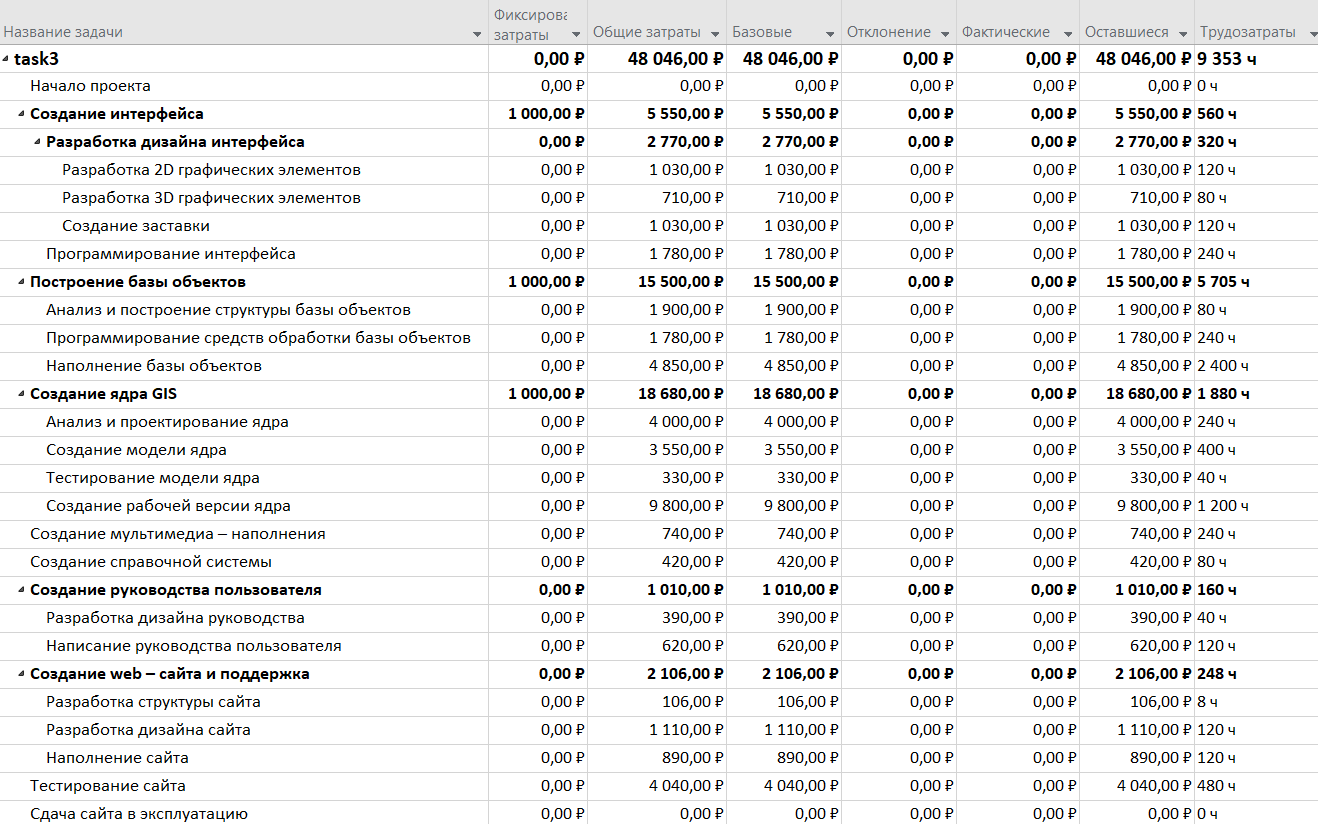
\includegraphics[width=1\linewidth]{inc/img/9.png}
	\caption{сопоставление в логике «Деньги» – «Объем работ»}
	\label{p9}
\end{figure}

\section*{Выводы}
По полученным диаграммам, можно сделать вывод, что программисты получают больше всего (50,13\%), а работают всего 29,08\%, в то время как наборщики данных работают аж 25,66\%, но получают только 10,77\%. Кроме этого, аренда дополнительного сервера, будет стоить 13,25\% от всех затрат, что заставляет задуматься над альтернативными решениями (например, самим сделать сервер).

По итогу проделанной работы выяснилось что выполнение проекта укладывается в отведенный бюджет 50 000 рублей, а также были освоены возможности программы Microsoft Project для работы с ресурсами.